\documentclass{article}
\usepackage[utf8]{inputenc}
\usepackage{graphicx}
\usepackage{fancyhdr}
\usepackage{hyperref}

% Set the page margins
\usepackage[margin=0.65in]{geometry} % narrower margins

\hypersetup{
    colorlinks=true,
    linkcolor=blue,
    filecolor=magenta,
    urlcolor=blue,
    citecolor=blue,
    pdfpagemode=FullScreen,
}

% Define header with university logo
\pagestyle{fancy}
\fancyhf{}
\lhead{
\includegraphics[width=2cm]{FAU-Logo.png}} 
\rhead{\textbf{Methods of Advanced Data Engineering (MADE), SoSe-2024} \\ \rule{\textwidth}{0.4pt}} 
\renewcommand{\headrulewidth}{0pt}


\begin{document}

% First Page
\begin{center}
    {\scshape\Large Data Report \par}
    \vspace{0.1cm}
    {\Large Prepared by: Redwanul Karim [\bf{23426184}] \par}
    \vspace{0.1cm} % You can remove this line if unnecessary
\end{center}

% Content Pages
\section{Introduction}
The project aims to explore the possible connection between solar activity - like solar flares, and climate change on Earth. Through the statistical analysis of historical data, our goal is to uncover whether there exists a clear relationship between solar events and the observable shift in global climate patterns. This investigation holds significant importance as it provides insights essential for refining climate models and improving our capacity to forecast and address the consequences of climate change. 

\section{Research Question}
\textbf{\textit{``Is there any relationship between solar activity (Solar Flares) and climate change on Earth?"}}

\section{Data Sources}

\subsection{Solar Flare Data}
   \begin{itemize}
       \item \textbf{Source:} Zenodo [\href{https://zenodo.org/records/4603412}{Dataset Link}]
       \item \textbf{Rationale:} The Solar Flare Dataset from Zenodo, comprising 8,874 records spanning from May 2010 to December 2019, provides crucial insights derived from vector magnetic field data collected by Joint Science Operations Center (JSOC) and the Space Weather Prediction Center (SWPC) using Python’s Sunpy library.
       \item \textbf{Data Content:} Recording Time, Flare Number, Lattitute, Longitude, Vector Magnetic Field data, such as - USFLUX, TOTPOT, TOTBSQ, ABSNJZH, and SAVNCPP etc.
       \item \textbf{Data Structure and Quality:} Tabular format (CSV), sourced from reliable JSOC and SWPC 
       \item \textbf{Licensing:} \href{https://opensource.org/license/MIT}{MIT License}
   \end{itemize}

\subsection{Temperature Change Data}
   \begin{itemize}
       \item \textbf{Source:} Annual Surface Temperature Change from IMF [\href{https://climatedata.imf.org/datasets/4063314923d74187be9596f10d034914/explore}{Dataset Link}]
       \item \textbf{Rationale:} The Surface Temperature Change dataset, obtained from Food and Agriculture Organization Corporate Statistical Database (FAOSTAT), shows how Earth's average surface temperature has changed from 1961 to 2021 compared to temperatures between 1951 and 1980, using data from NASA GISS. It helps analyze temperature changes in different countries and is essential for understanding global temperature patterns.
       \item \textbf{Data Content:} Date, Country, ISO3, Temperature change etc.
       \item \textbf{Data Structure and Quality:} Tabular format (CSV), sourced from FAOSTAT 
       \item \textbf{Licensing:} \href{https://www.imf.org/external/terms.htm}{IMF License}
   \end{itemize}

\subsection{CO$_2$  Concentration Data}
   \begin{itemize}
       \item \textbf{Source:} Atmospheric CO$_2$ Concentrations from IMF [\href{https://climatedata.imf.org/datasets/9c3764c0efcc4c71934ab3988f219e0e/explore}{Dataset Link}]
       \item \textbf{Rationale:} The Atmospheric CO$_2$ dataset offers monthly and yearly records of carbon dioxide levels in the air dating back to 1958, enabling users to track changes over time. Sourced from the National Oceanic and Atmospheric Administration Global Monitoring Laboratory, that provides dependable data crucial for climate research and analysis.
       \item \textbf{Data Content:} Date, CO$_2$ Concentration in PPM etc.
       \item \textbf{Data Structure and Quality:} Tabular format (CSV), sourced from NOAA 
       \item \textbf{Licensing:} \href{https://www.imf.org/external/terms.htm}{IMF License}
   \end{itemize}

\section{Data Pipeline}

In this section, we describe the ETL (Extract, Transform, Load) data pipeline implemented for our project. The pipeline is designed to systematically download, process, and store data from various sources, ensuring it is clean, structured, and ready for analysis. Below, we detail each step of the ETL Data Pipeline.

\begin{figure}[h]
    \centering
    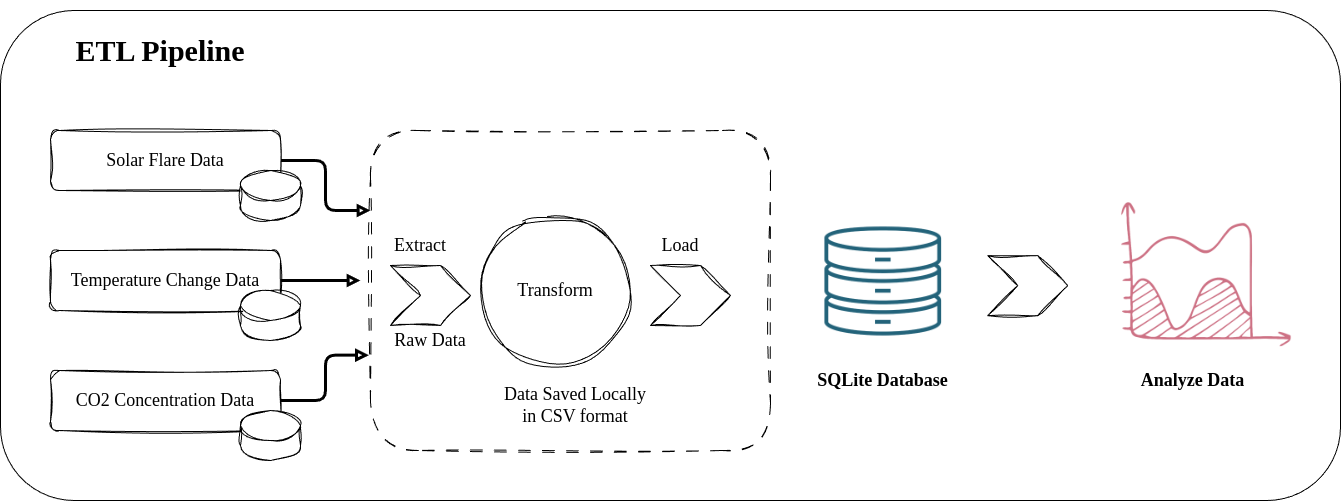
\includegraphics[width=1\textwidth]{ETL.png} % Replace 'example-image' with your image filename
    \caption{ETL Data Pipeline}
    \label{fig:example}
\end{figure}

\subsection{Extract}

The extraction phase involves sourcing datasets from their respective origins. The datasets used include Solar Flare Data, Temperature Change Data, and CO$_2$ Concentration Data. Using Pandas' CSV reader, we downloaded these datasets and saved them locally as CSV files. This method ensures data is captured in a structured and accessible format for subsequent processing.

\subsection{Transform}
The transformation phase involves several key steps to clean and prepare the data for analysis:

\begin{itemize}
    \item \textbf{Data Ingestion and Cleaning:} The locally saved CSV files are read into Pandas DataFrames, as it provides a flexible structure for data manipulation. Unnecessary columns such as - Indicator, Unit, Source, CTS Code, CTS Full Descriptor etc, are removed as these data do not contribute to the analysis phase, and rows with missing values are dropped to ensure data integrity.
    \item \textbf{Data Type Conversion:} Columns representing dates and times are converted to appropriate datetime formats, and columns are renamed for clarity and consistency, for example column `T\_REC' in Solar Flare data was renamed to `Date'.
    \item \textbf{Data Reshaping:} Using Pandas' melt method, wide-format temperature change data is converted into long-format, transforming columns into rows. This normalization step makes the data easier to work with for analysis and storage.
    \item \textbf{Saving Transformed Data:} The cleaned and transformed data points are saved back to local CSV files, that provides a checkpoint before loading into the SQLite database.
\end{itemize}


\subsection{Load}

The loading phase involves importing the transformed data into a structured database format. A SQLite database is created to store the transformed data due to its simplicity and ease of integration with Pandas. The transformed CSV files are read into Pandas DataFrames again, and each DataFrame is loaded into its own table within the SQLite database. This separation ensures organized and efficient data storage, enabling straightforward querying and analysis.

By following these ETL steps, the data pipeline effectively extracts, transforms, and loads datasets, making them ready for further analysis and ensuring high data quality and consistency throughout the process.

\section{Data Analysis}

We conducted a statistical analysis to investigate the relationship between solar activity (Solare Flare events) and climate change (Temperature Change and CO$_2$ concentration) on Earth. Using a subset of our data extracted from the sink SQLite database prepared with the ETL Data Pipeline. 

We began by determining the common time window for all datasets and then employed a Random Forest Regressor to identify the top 5 significant features from the Solar Flare dataset, namely 'TOTBSQ', 'TOTPOT', 'ABSNJZH', 'SAVNCPP', and 'USFLUX'. Subsequently, we performed hypothesis testing using t-tests for Temperature change and CO$_2$ concentration, revealing significant p-values for both variables.

\begin{figure}[h]
    \centering
    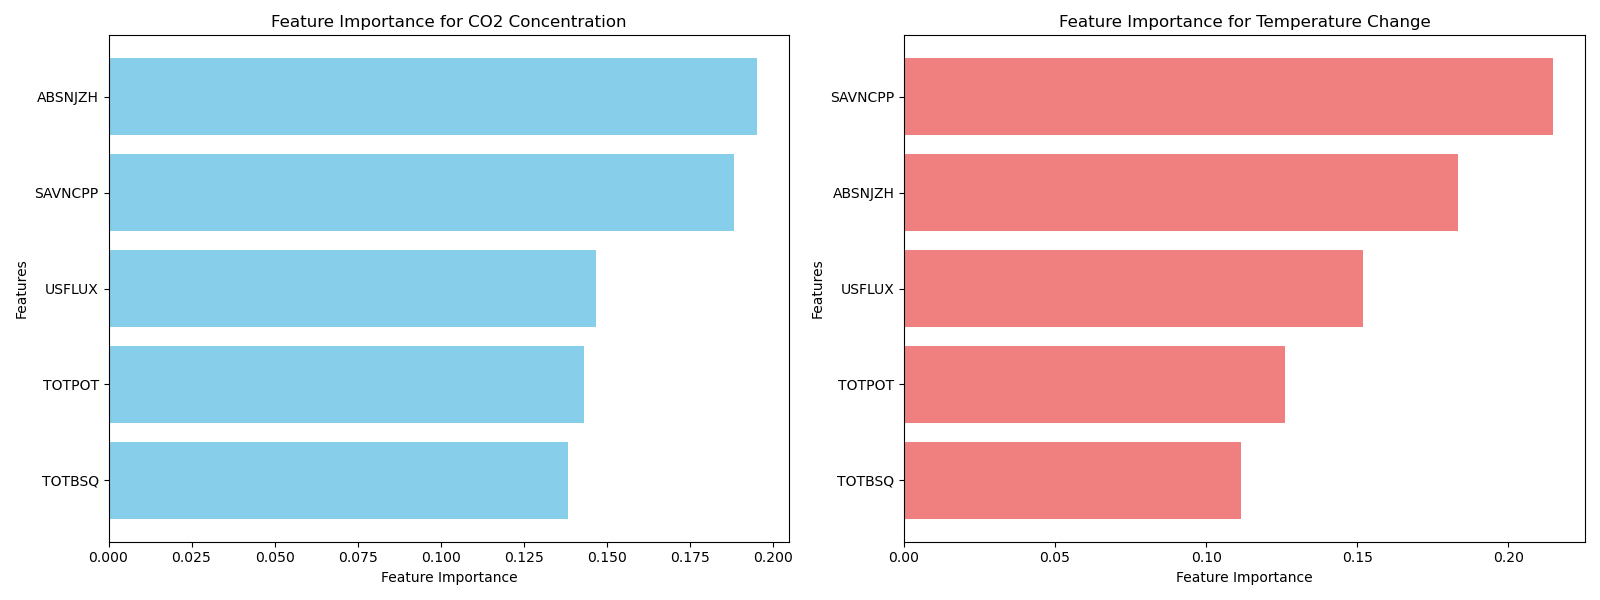
\includegraphics[width=0.7\textwidth]{feature_importance_plot.png} % Replace 'example-image' with your image filename
    \caption{Five most important feature of Solar Flare data in relation to Temperature Change and CO$_2$ Concentration on Earth}
    \label{fig:example}
\end{figure}

\section{Result}

The hypothesis testing (t-tests) revealed notable p-values for both CO$_2$ concentration and Temperature change. However, a deeper examination on data distribution and auto-correlation of the data variables uncovered that the data points we are using violates the underlying assumptions of normality and homogeneity of variances, which casts a doubt on the validity of our hypothesis testing results. As a result, based on our data analysis, at this point we cannot conclude with certainty that there is relationship between solar flare events and climate change on earth.

\begin{figure}[h]
    \centering
    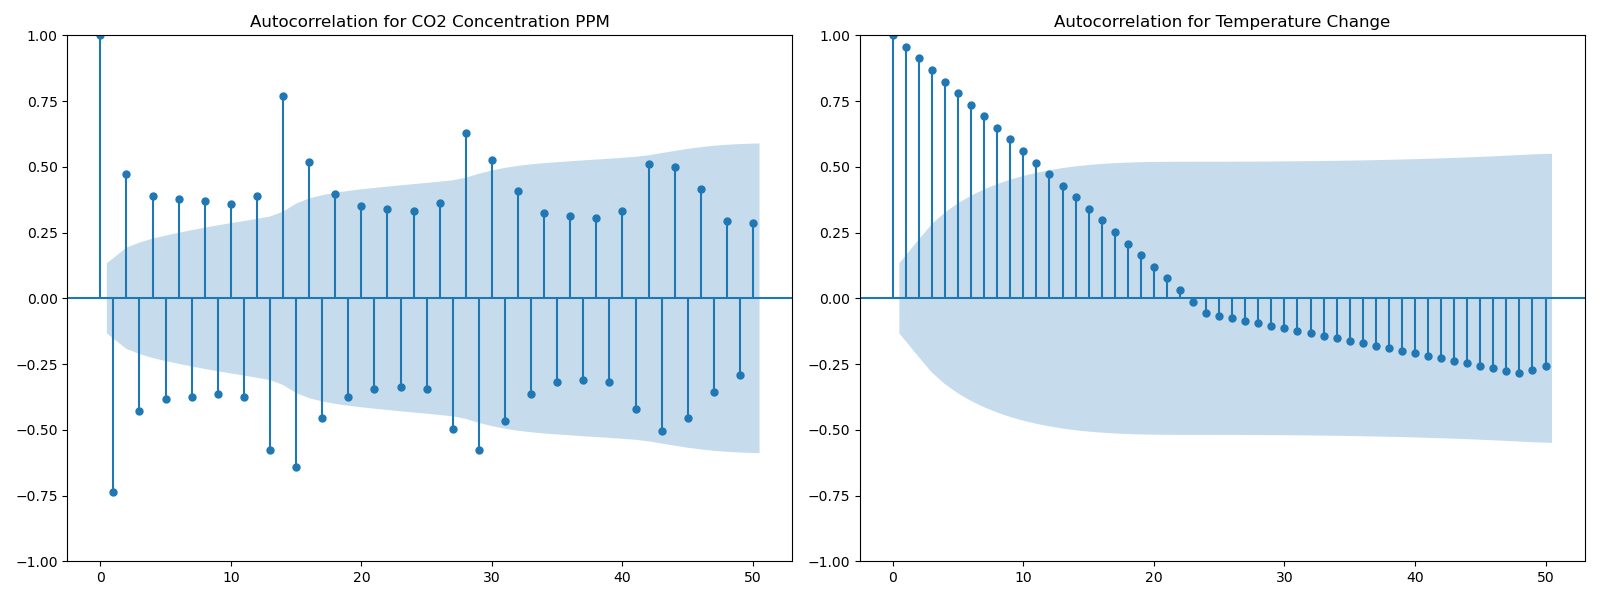
\includegraphics[width=0.7\textwidth]{autocorrelation_plots.png} % Replace 'example-image' with your image filename
    \caption{Auto-correlation plot of Temperature Change and CO$_2$ Concentration data}
    \label{fig:example}
\end{figure}

\section{Limitations and Future Direction}

While hypothesis testing offers useful information about statistical correlations, it doesn't prove cause and effect. Additionally, the violations of assumptions like normality and equal variances mean we should be careful with our interpretations. Moving forward, we need to explore domain-specific machine learning algorithms to handle the complexities of non-normally distributed data in order to better understand the relationship between solar activity and climate change on Earth.

\end{document}
